\documentclass{standalone}
\usepackage{pgfplots}
\pgfplotsset{compat=1.18}

\begin{document}

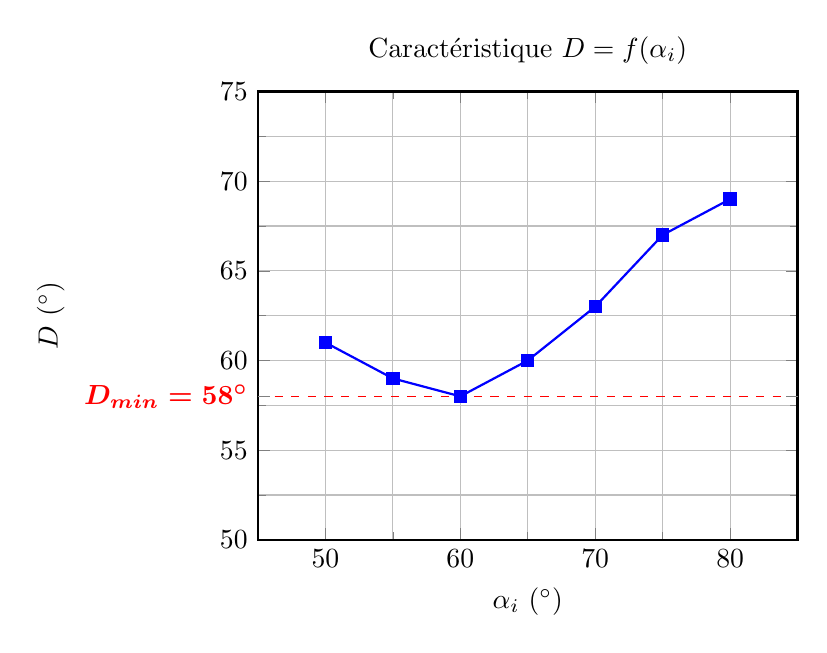
\begin{tikzpicture}
\begin{axis}[
    title={Caractéristique $D = f(\alpha_i)$},
    xlabel={$\alpha_i$ ($^{\circ}$)},
    ylabel={$D$ ($^{\circ}$)},
    grid=both,
    minor tick num=1,
    xmin=45, xmax=85,
    ymin=50, ymax=75, % J'ai baissé ymin pour bien voir la projection au sol
    thick,
    % --- Ajout des valeurs spécifiques sur les axes ---
    extra y ticks={58},
    extra y tick labels={$D_{min} = 58^{\circ}$},
    extra tick style={grid=major, tick label style={text=red, font=\boldmath}, grid style={dashed, red}}
]
    \addplot[
        color=blue,
        mark=square*,
    ] coordinates {
        (50, 61) (55, 59) (60, 58) (65, 60) (70, 63) (75, 67) (80, 69)
    };
    
    % Le point sur la courbe
    \node[fill=red, circle, inner sep=1.5pt] at (axis cs:60, 58) {};
    
\end{axis}
\end{tikzpicture}

\end{document}